\originalchapter{作业九：辐射、声子与 Johnson 噪声}
\psource{8.044，2013 春，PS9，4 月 19 日截止。中文题面；据官方答案核对的 AI 独立解答。原题交叉引用沿用旧编号，以下明确改为本卷实际第 3、4 题。}
\originalsection{1．宇宙辐射的绝热尺度}
\begin{exercise}
辐射与物质在约 3000 K 脱耦，题设如今黑体温度 3 K。假定绝热膨胀，体积增至多少倍、相对增加多少？可用 $F=-\pi^2V(\kb T)^4/(45\hbar^3c^3)$。这些温度为原题近似数值；局域恒星辐射仍可与物质平衡。
\end{exercise}
\begin{solution}
$S=-F_T\propto VT^3$，固定熵给 $V_f/V_i=(3000/3)^3=10^9$，相对增加 $(V_f-V_i)/V_i=10^9-1$。该体积指同一共动辐射块的尺度，非有限“宇宙边界”的测量。
\end{solution}
\originalsection{2．固体晶格热容}
\begin{exercise}
晶体有 $N$ 个原胞、每胞 $J$ 个原子。
(a) 经典独立原子各三个谐振方向，至多 $3J$ 种频率，求恒体积热容；
(b) Einstein 模型各频率同为 $\nu$，量子计算热容及 $\kb T\ll h\nu$、$\kb T\gg h\nu$ 极限；
(c) 耦合原子构成 $3JN$ 个正常模，$\int D(\omega)\dd\omega=3JN$。(i) 写完整内能积分并取高于全部频率的温度极限；(ii) 低频 $D(\omega)=3V\omega^2/(2\pi^2\avg v^3)$，低温仅此区域被激发，求热容，可用 $\int_0^\infty x^3/(e^x-1)\dd x=\pi^4/15$。原题的外书测量图已分离，MIT 问题与此数据条件完整保留。
\end{exercise}
\begin{solution}
(a) 每模动能、势能各 $\kb T/2$，$C_V=3JN\kb$。
(b) 令 $x=h\nu/(\kb T)$，$C_V=3JN\kb x^2e^x/(e^x-1)^2$；低温 $3JN\kb x^2e^{-x}$，高温 $3JN\kb$。
(c)(i) $U=\int_0^\infty\hbar\omega[1/2+(e^{\beta\hbar\omega}-1)^{-1}]D(\omega)\dd\omega$。高温总能主项 $3JN\kb T$、热容同经典；零点项不贡献恒体积热容。(ii) 热激发能 $U_T=\pi^2V(\kb T)^4/(10\hbar^3\avg v^3)$，所以 $C_V=2\pi^2V\kb^4T^3/(5\hbar^3\avg v^3)$。有效速度满足 $3/\avg v^3=1/v_L^3+2/v_T^3$，并非普通算术平均。
\end{solution}
\originalsection{3．储能元件的热噪声}
\begin{exercise}
任意无源被动网络与温度 $T$ 热库平衡。(a) 电容 $C$ 的电压密度和均方根；$T=300$ K、$C=100$ pF 时以微伏算；(b) 电感 $L$ 的电流密度和均方根，$L=1$ mH 时以纳安算；(c) 为什么此方法不能给电阻电压？
\end{exercise}
\begin{solution}
电容能 $Cv^2/2$ 给 $p(v)=\sqrt{C/(2\pi\kb T)}e^{-Cv^2/(2\kb T)}$、$v_{\rm rms}=\sqrt{\kb T/C}=6.436$ 微伏。电感能 $Li^2/2$ 同理 $p(i)=\sqrt{L/(2\pi\kb T)}e^{-Li^2/(2\kb T)}$、$i_{\rm rms}=\sqrt{\kb T/L}=2.035$ 纳安。电阻耗散而不以 $Rv^2/2$ 储能，电压噪声须给带宽和周围阻抗。这里采用经典可达独立储能坐标，受额外电路约束时应先选独立正常坐标。
\end{solution}
\originalsection{4．由传输线求噪声功率}
\begin{exercise}
真空同轴 TEM 线长 $L$，两端短路，单电压偏振，$\omega=ck$。
(a) 允许波数；(b) 大量模式时 $D(\omega)$；(c) 热平衡每长度每角频率的能量 $u_1(\omega,T)$；(d) $\kb T\gg\hbar\omega$ 极限；(e) 线切开并接匹配电阻，行波一半入射、完全吸收；细致平衡求电阻每角频率向线发出功率；(f) 室温 300 K、普通频率带宽 10 MHz 内的功率。积分采用正角频率 $0<\omega<\infty$，不重复计负频率。
\end{exercise}
\begin{solution}
(a) $k_n=n\pi/L$，$n=1,2,\ldots$。(b) $D=L/(\pi c)$。(c) 模式总能量密度 $u_{1,\rm total}=\hbar\omega[1/2+(e^{\beta\hbar\omega}-1)^{-1}]/(\pi c)$；扣去真空零点后热能 $u_{1,\rm th}=\hbar\omega/[\pi c(e^{\beta\hbar\omega}-1)]$。(d) 为 $\kb T/(\pi c)$。(e) 热能入射单向通量 $cu_{1,\rm th}/2$，所以经典 $P_\omega=\kb T/(2\pi)$，与匹配阻值无关。(f) $\Delta\omega=2\pi\Delta\nu$，$P=\kb T\Delta\nu=4.142\times10^{-14}$ W。白谱仅在经典低频窗口成立。
\end{solution}
\originalsection{5．实际电阻与 RC 谱}
\begin{exercise}
以理想电阻 $R$ 串联随机电压源 $v_N$ 表示真实电阻。
(a) 连到输入阻抗同为 $R$ 的匹配线，求每频率功率与 $\avg{v_N^2(\omega)}$ 关系；(b) 与第 4(e) 题相等，证明单边角频谱 $S_N=2R\kb T/\pi$；(c) RC 串联电路在电容上的传递功率因子 $1/[1+(RC\omega)^2]$，求并画 $S_C(\omega)$，积分求总均方根，与第 3(a) 题比较。
\end{exercise}
\begin{solution}
(a) 分压后二分之一电压，线得 $P_\omega=S_N/(4R)$。(b) 令其等于 $\kb T/(2\pi)$ 得所求谱。(c) $S_C=2R\kb T/[\pi(1+(RC\omega)^2)]$，在 $\omega_c=1/(RC)$ 降半，尾随 $\omega^{-2}$；$\int_0^\infty S_C\dd\omega=\kb T/C$，与储能方法一致。转换成每 Hz 单边源谱为 $4R\kb T$。
\end{solution}
\begin{center}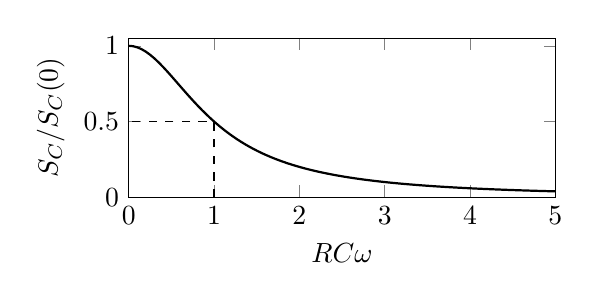
\begin{tikzpicture}\begin{axis}[width=7cm,height=3.6cm,xmin=0,xmax=5,ymin=0,ymax=1.05,xlabel={$RC\omega$},ylabel={$S_C/S_C(0)$},samples=100]\addplot[domain=0:5,thick]{1/(1+x*x)};\draw[dashed](axis cs:1,0)--(axis cs:1,.5)--(axis cs:0,.5);\end{axis}\end{tikzpicture}\end{center}
